\documentclass{article}
\usepackage[utf8]{inputenc}
\usepackage{graphicx}
\usepackage{float}
\usepackage{amsmath}
\usepackage[paper=a4paper,margin=1in]{geometry}
\usepackage[table,xcdraw]{xcolor}
\usepackage{url}

\title{Image classification with CNNs}
\author{David Štych\\ Aleksandra Jamróz}
\date{\today{}}



\begin{document}
\maketitle



\section*{Baseline performance}
Firstly, let us define a baseline to beat. We run the provided code with a 500 dataset size for 25 epochs. Maximum AUC was \textbf{0.804709} after 10 epochs. Then the model stopped improving noticeably.
\begin{figure}[H]
\centering
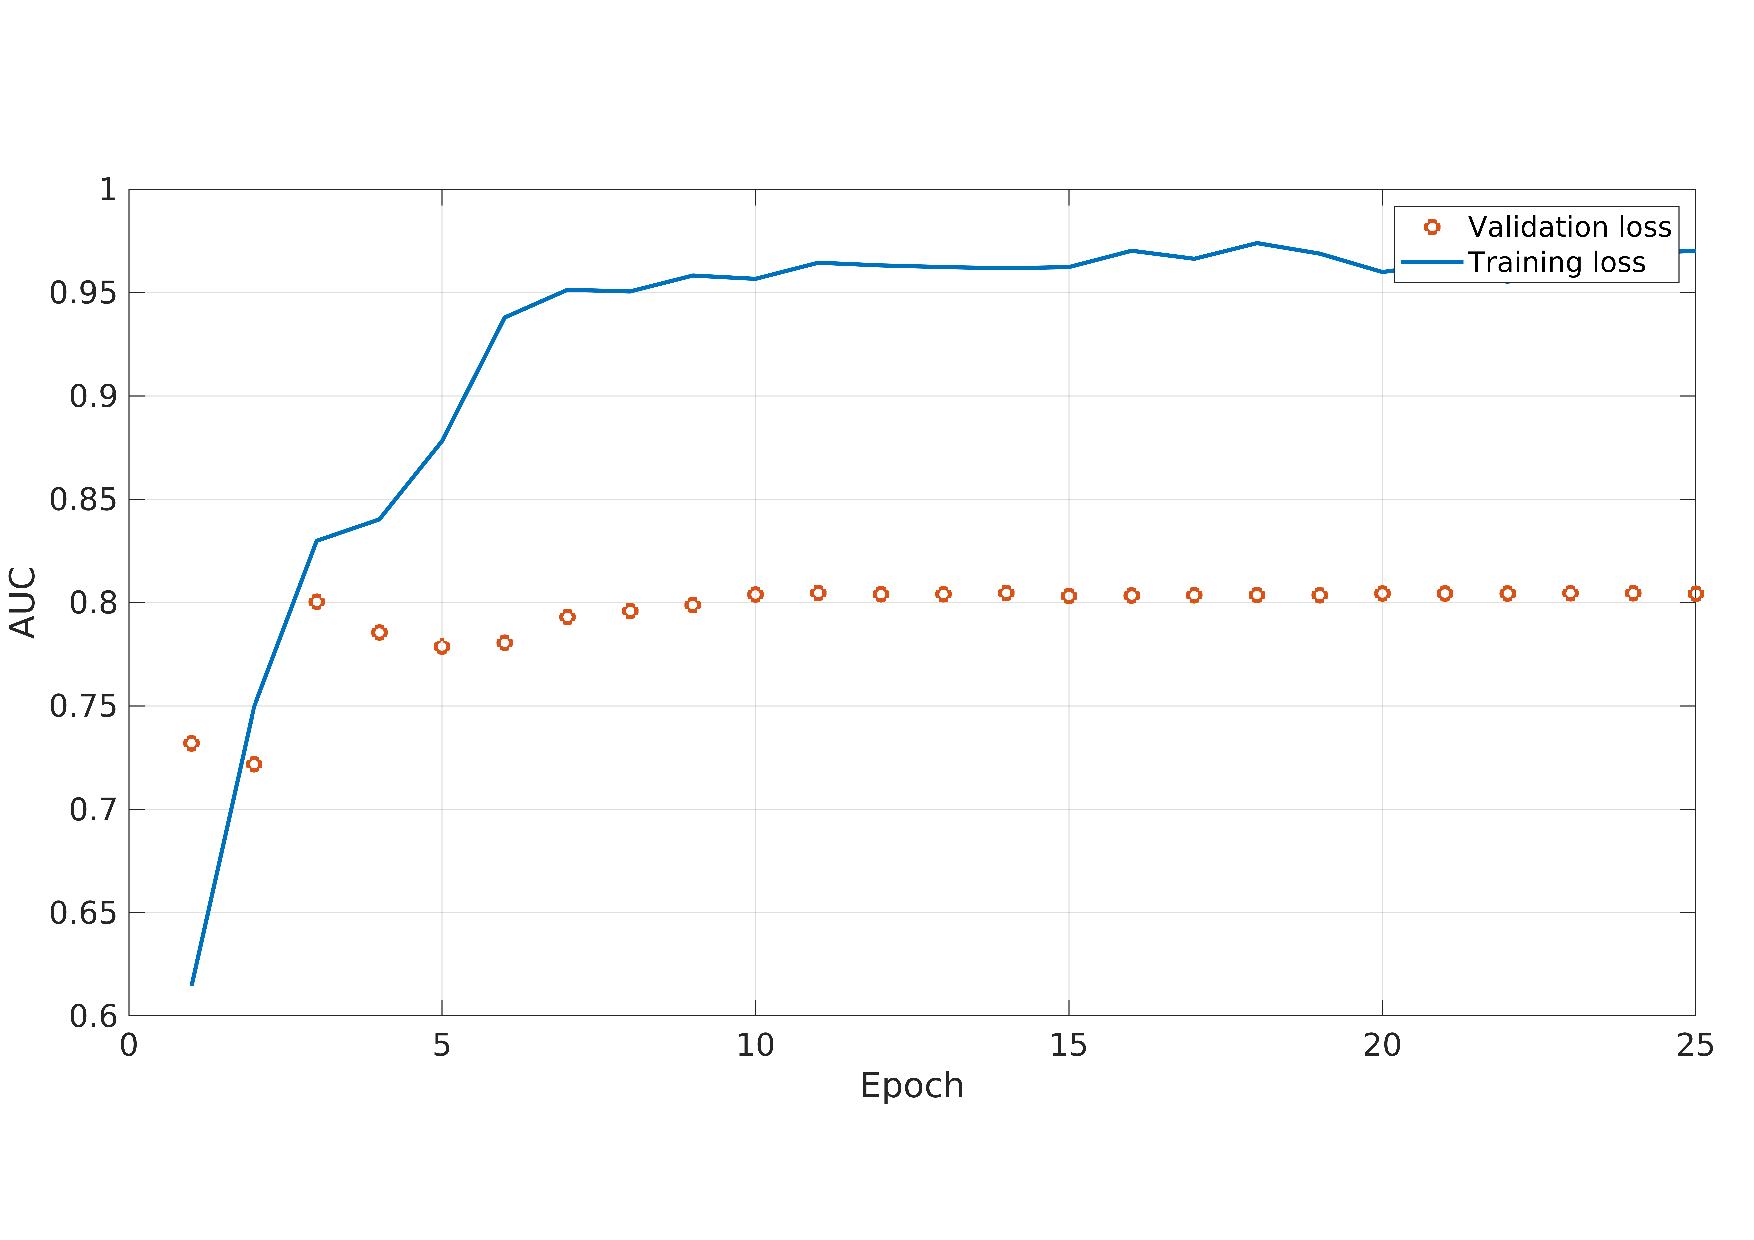
\includegraphics[width=0.85\textwidth]{figures/default_AUC_progress.pdf}
\caption{Default model - average AUC progress during learning}
\end{figure}


\section*{Improvements}

\begin{itemize}
\item We have used data augmentation to randomize training data to reduce overfitting and achieve better performance \cite{somewebsite}

To the training dataset, we applied the following transformations: 
\begin{itemize}
\item Random rotation of the image by $\pm30^{\circ}$

\textit{torchvision: RandomRotation} \cite{randomrotation}
\item Crop a random portion of an image and resize it to a given size

\textit{torchvision: RandomResizedCrop} \cite{randomresizedcrop}
\item Randomly flipping the image horizontally with a probability of 50\%

\textit{torchvision: RandomHorizontalFlip} \cite{randomhorizontalflip}
\item Converting to PyTorch tensor and normalization
\end{itemize} 
To the validation and test dataset, we applied the following transformations: 
\begin{itemize}
\item Resize the image to a specific size

\textit{torchvision: Resize} \cite{resize}
\item Crop the image at the center to a specific size

\textit{torchvision: CenterCrop} \cite{centercrop}
\item Converting to PyTorch tensor and normalization
\end{itemize}       
\item Class balancing


%\begin{table}[H]
%\centering
%\begin{tabular}{|
%>{\columncolor[HTML]{FFFFFF}}c |c|}
%\hline
%\cellcolor[HTML]{C0C0C0}{\color[HTML]{000000} \textbf{Label}} & \cellcolor[HTML]{C0C0C0}{\color[HTML]{000000} \textbf{Number of %samples in the dataset}} \\ \hline
%{\color[HTML]{000000} nevus}                                  & {\color[HTML]{000000} 1372}                                                              %\\ \hline
%{\color[HTML]{000000} melanoma}                               & {\color[HTML]{000000} 374}                                                               %\\ \hline
%{\color[HTML]{000000} keratosis}                              & {\color[HTML]{000000} 254}                                                               %\\ \hline
%\end{tabular}
%\end{table}


\begin{figure}[H]
\centering
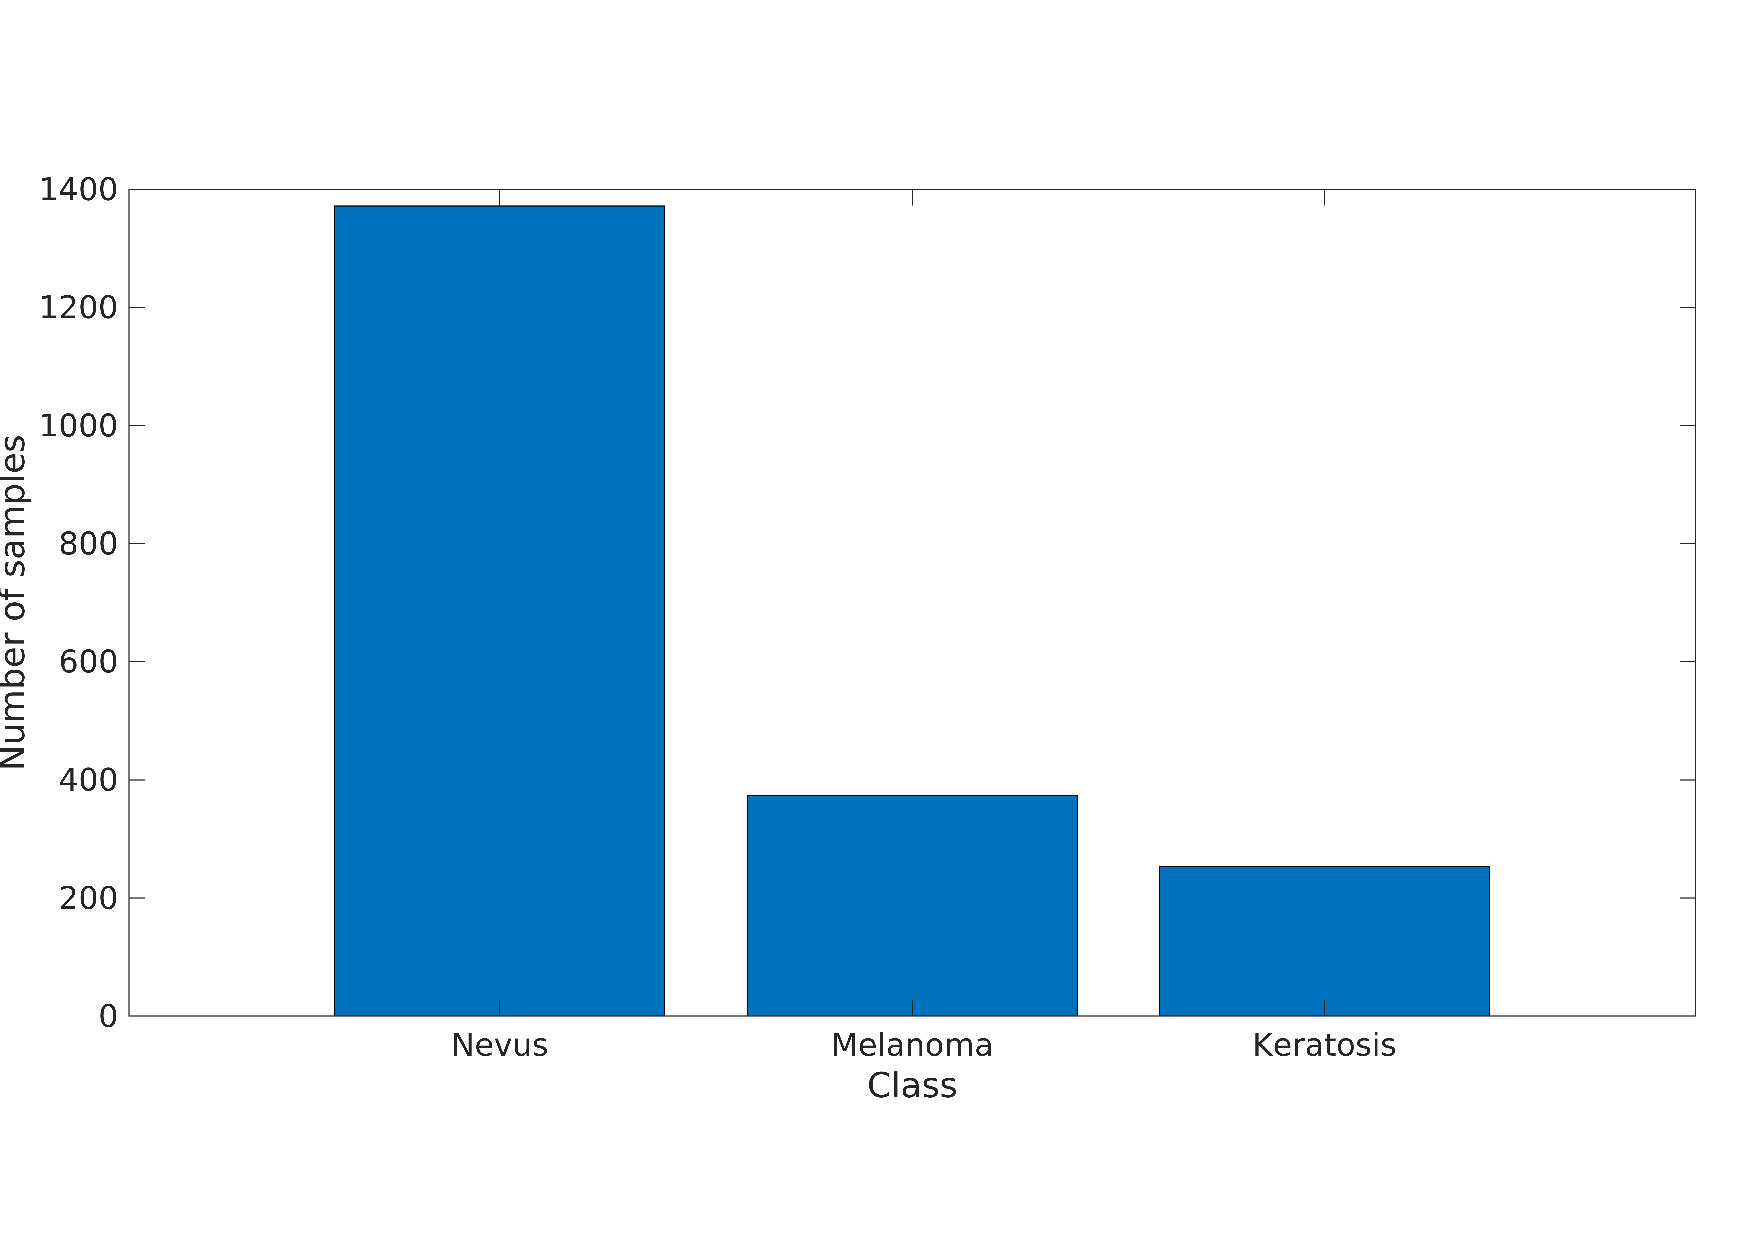
\includegraphics[width=0.75\textwidth]{figures/class_distribution.pdf}
\caption{Dataset class distribution}
\end{figure}


The figure above shows the sample distribution in the dataset. Clearly, nevus is much more prevalent in the dataset, which is what we expect as it is a more common medical problem. \cite{wiki} Nevertheless, we used class weights as an argument in the loss function, leading to an improvement of the model. For each class, we calculated weight with the following formula: 
$$\text{Class weight}=1-\frac{\text{Number of samples in the dataset}}{\text{Total number of samples}}$$
\item We have used Adam optimizer resulting in faster learning. Selected learning rate = 0.0001.
\item We changed \textit{maxSize} argument to 0, meaning we have used the entire dataset. That was possible thanks to the Czech Technical University in Prague (the home university of one of the authors of this report), which allowed us to use their computational resources. \cite{ctu}
\end{itemize}


\section*{Conslusion}
\begin{figure}[H]
\centering
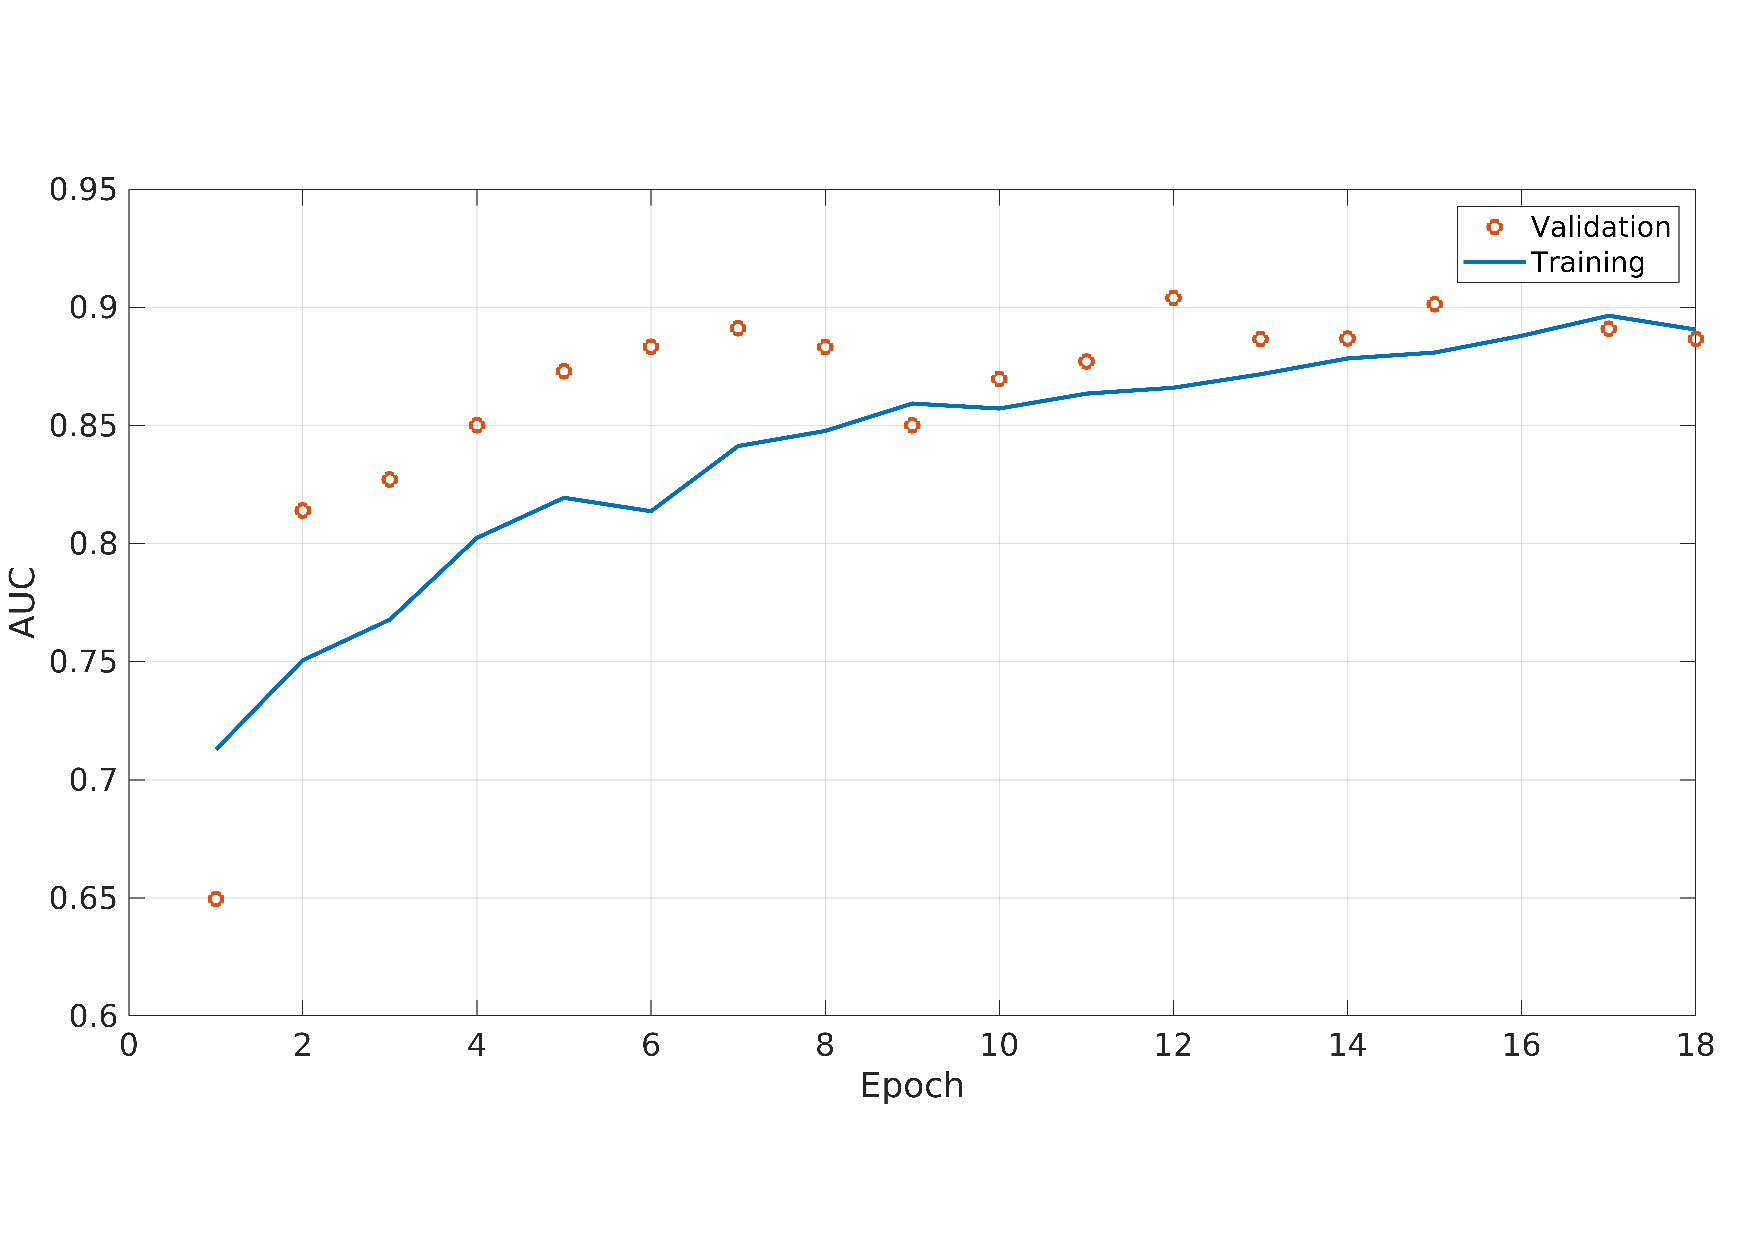
\includegraphics[width=\textwidth]{figures/progress_AUC_091.pdf}
\caption{Final model - average AUC progress during learning}
\end{figure}
The figure above shows the development of AUC during learning. We tried to train to model for more epochs, but no further improvement was noticed after 15-16 epochs.

Our best result was \textbf{0.913973} average AUC over the validation dataset.

\begin{table}[H]
\centering
\begin{tabular}{|l|c|c|c|}
\hline
\rowcolor[HTML]{C0C0C0} 
\multicolumn{1}{|c|}{\cellcolor[HTML]{C0C0C0}{\color[HTML]{000000} \textbf{Changes to the model}}}                                        & {\color[HTML]{000000} \textbf{\begin{tabular}[c]{@{}c@{}}AUC - binary problem\\ melanoma\end{tabular}}} & {\color[HTML]{000000} \textbf{\begin{tabular}[c]{@{}c@{}}AUC - binary problem\\ keratosis\end{tabular}}} & {\color[HTML]{000000} \textbf{\begin{tabular}[c]{@{}c@{}}AUC \\ Average\end{tabular}}} \\ \hline
\rowcolor[HTML]{FFFFFF} 
{\color[HTML]{000000} No changes - baseline}                                                                                           & {\color[HTML]{000000} 0.731111}                                                                         & {\color[HTML]{000000} 0.878307}                                                                         & {\color[HTML]{000000} 0.804709}                                                        \\ \hline
\rowcolor[HTML]{FFFFFF} 
{\color[HTML]{000000} \begin{tabular}[c]{@{}l@{}}Data augumentation\\ Using the entire dataset\\ Adam optimizer\end{tabular}}                    & {\color[HTML]{000000} 0.836389}                                                                         & {\color[HTML]{000000} 0.954806}                                                                         & {\color[HTML]{000000} 0.895597}                                                        \\ \hline
\rowcolor[HTML]{FFFFFF} 
{\color[HTML]{000000} \begin{tabular}[c]{@{}l@{}}Data augumentation\\ Using the entire dataset\\ Class balancing \\ Adam optimizer\end{tabular}} & {\color[HTML]{000000} 0.876667}                                                                         & {\color[HTML]{000000} 0.951279}                                                                         & {\color[HTML]{000000} \textbf{0.913973}}                                                        \\ \hline
\end{tabular}
\end{table}


\newpage

\bibliographystyle{unsrt}
\bibliography{references}








\end{document}

